\chapter{船岸连接系统结构与分析}

\zhlipsum[2]

\begin{figure}[!htp]
	\centering
	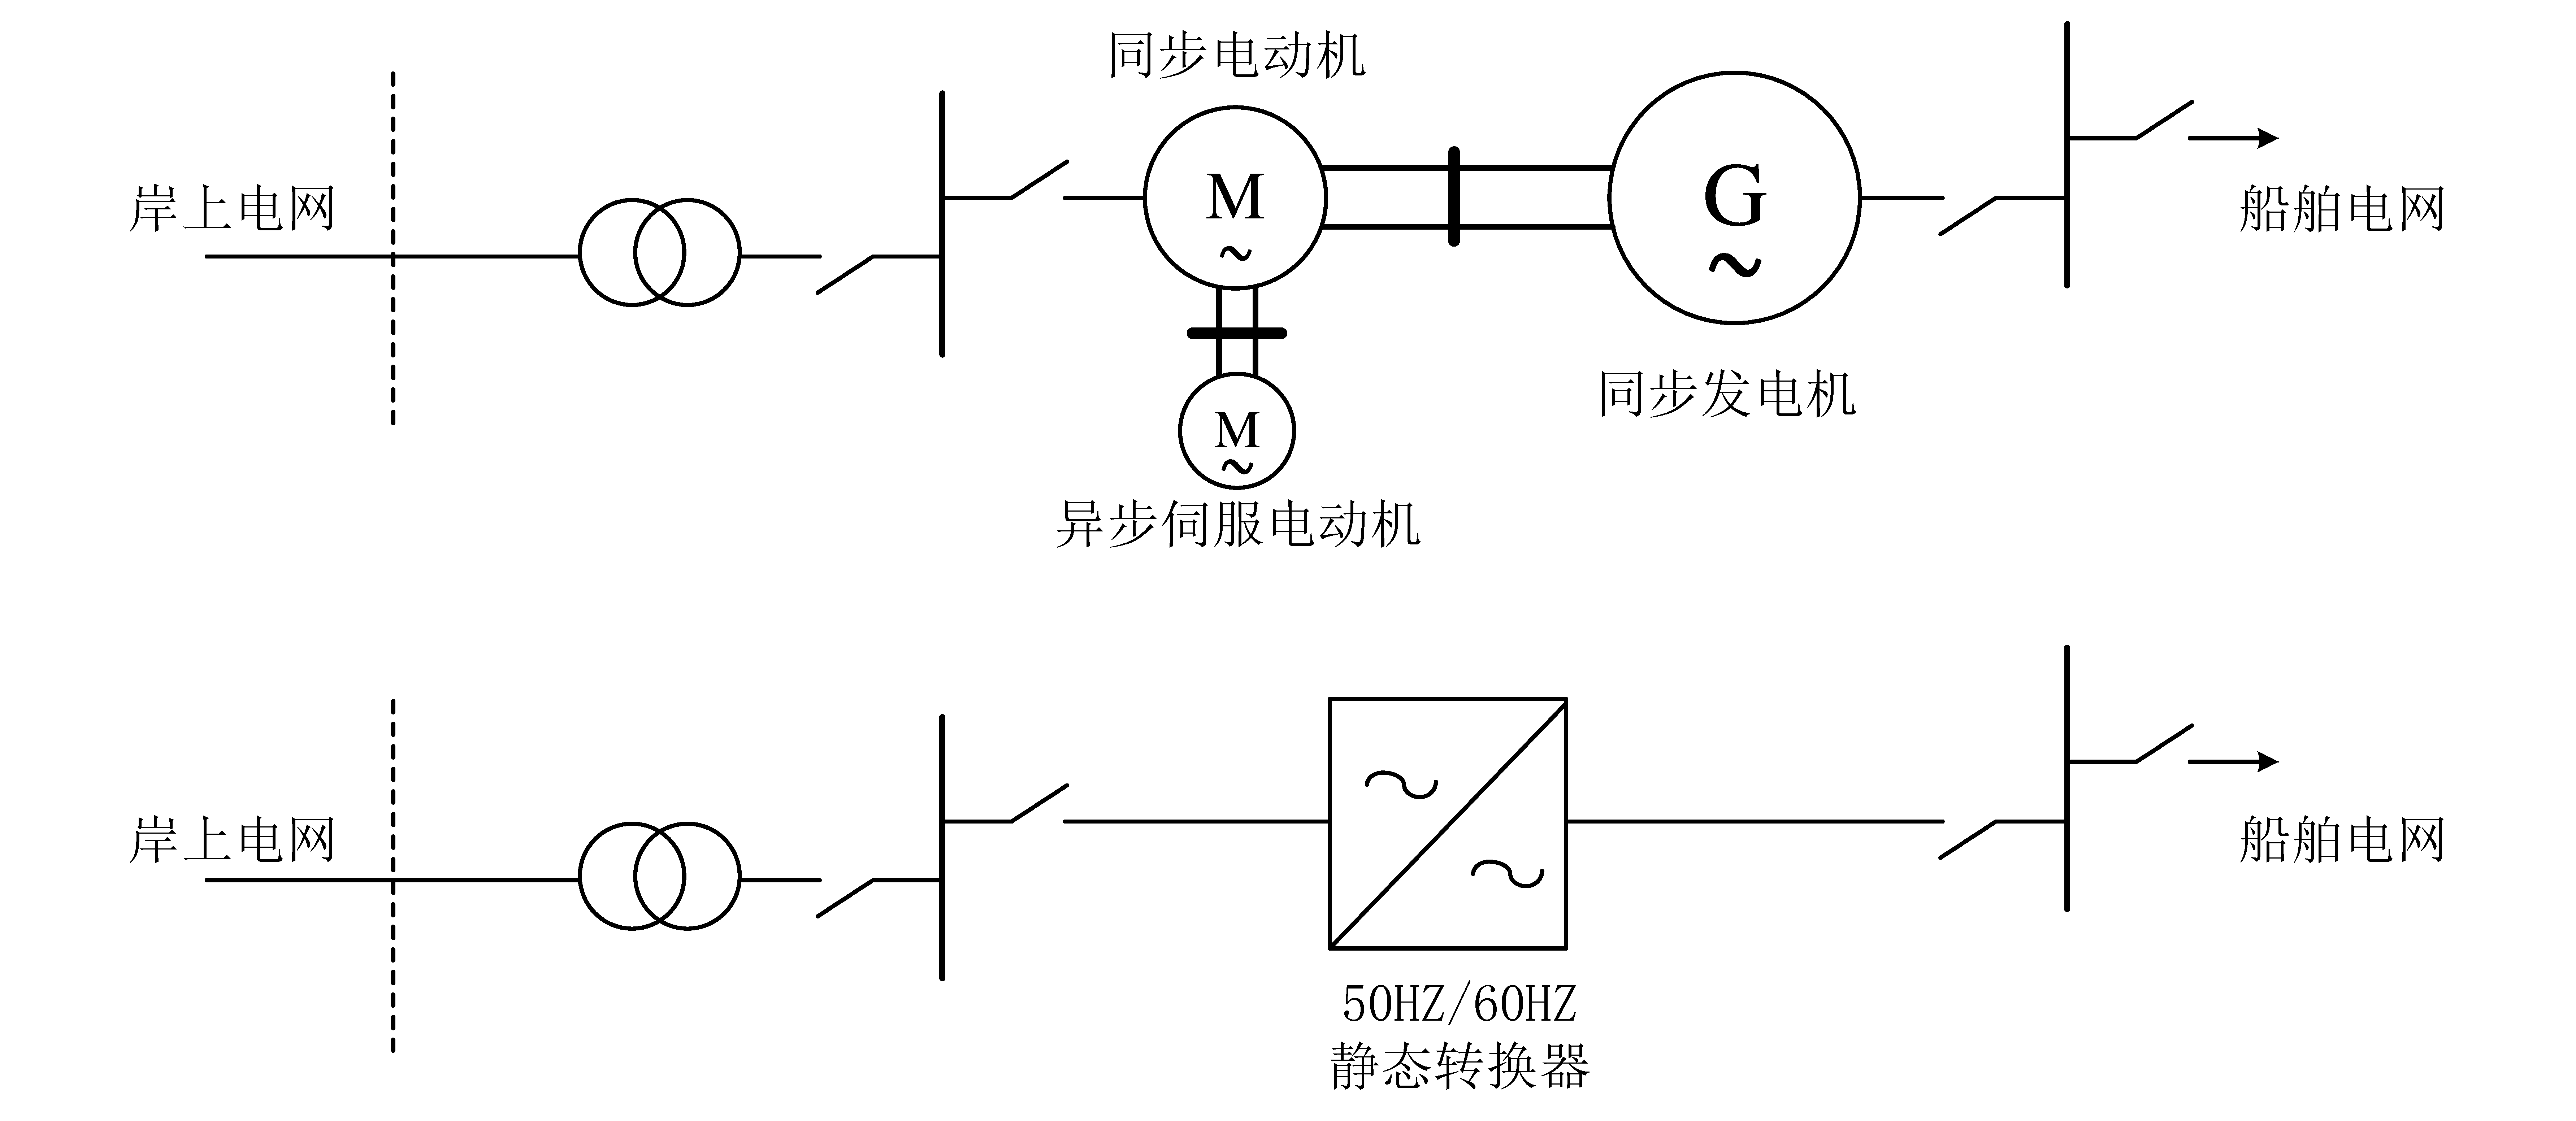
\includegraphics[width=0.85\textwidth]{旋转形态转换器对比.pdf}
	\caption{传统旋转变频与静态电源变频对比}
	\label{fig:传统旋转变频与静态电源变频对比}
\end{figure}



\section{船岸连接系统的组成}

\zhlipsum[3]

\begin{figure}[!htp]
	\centering
	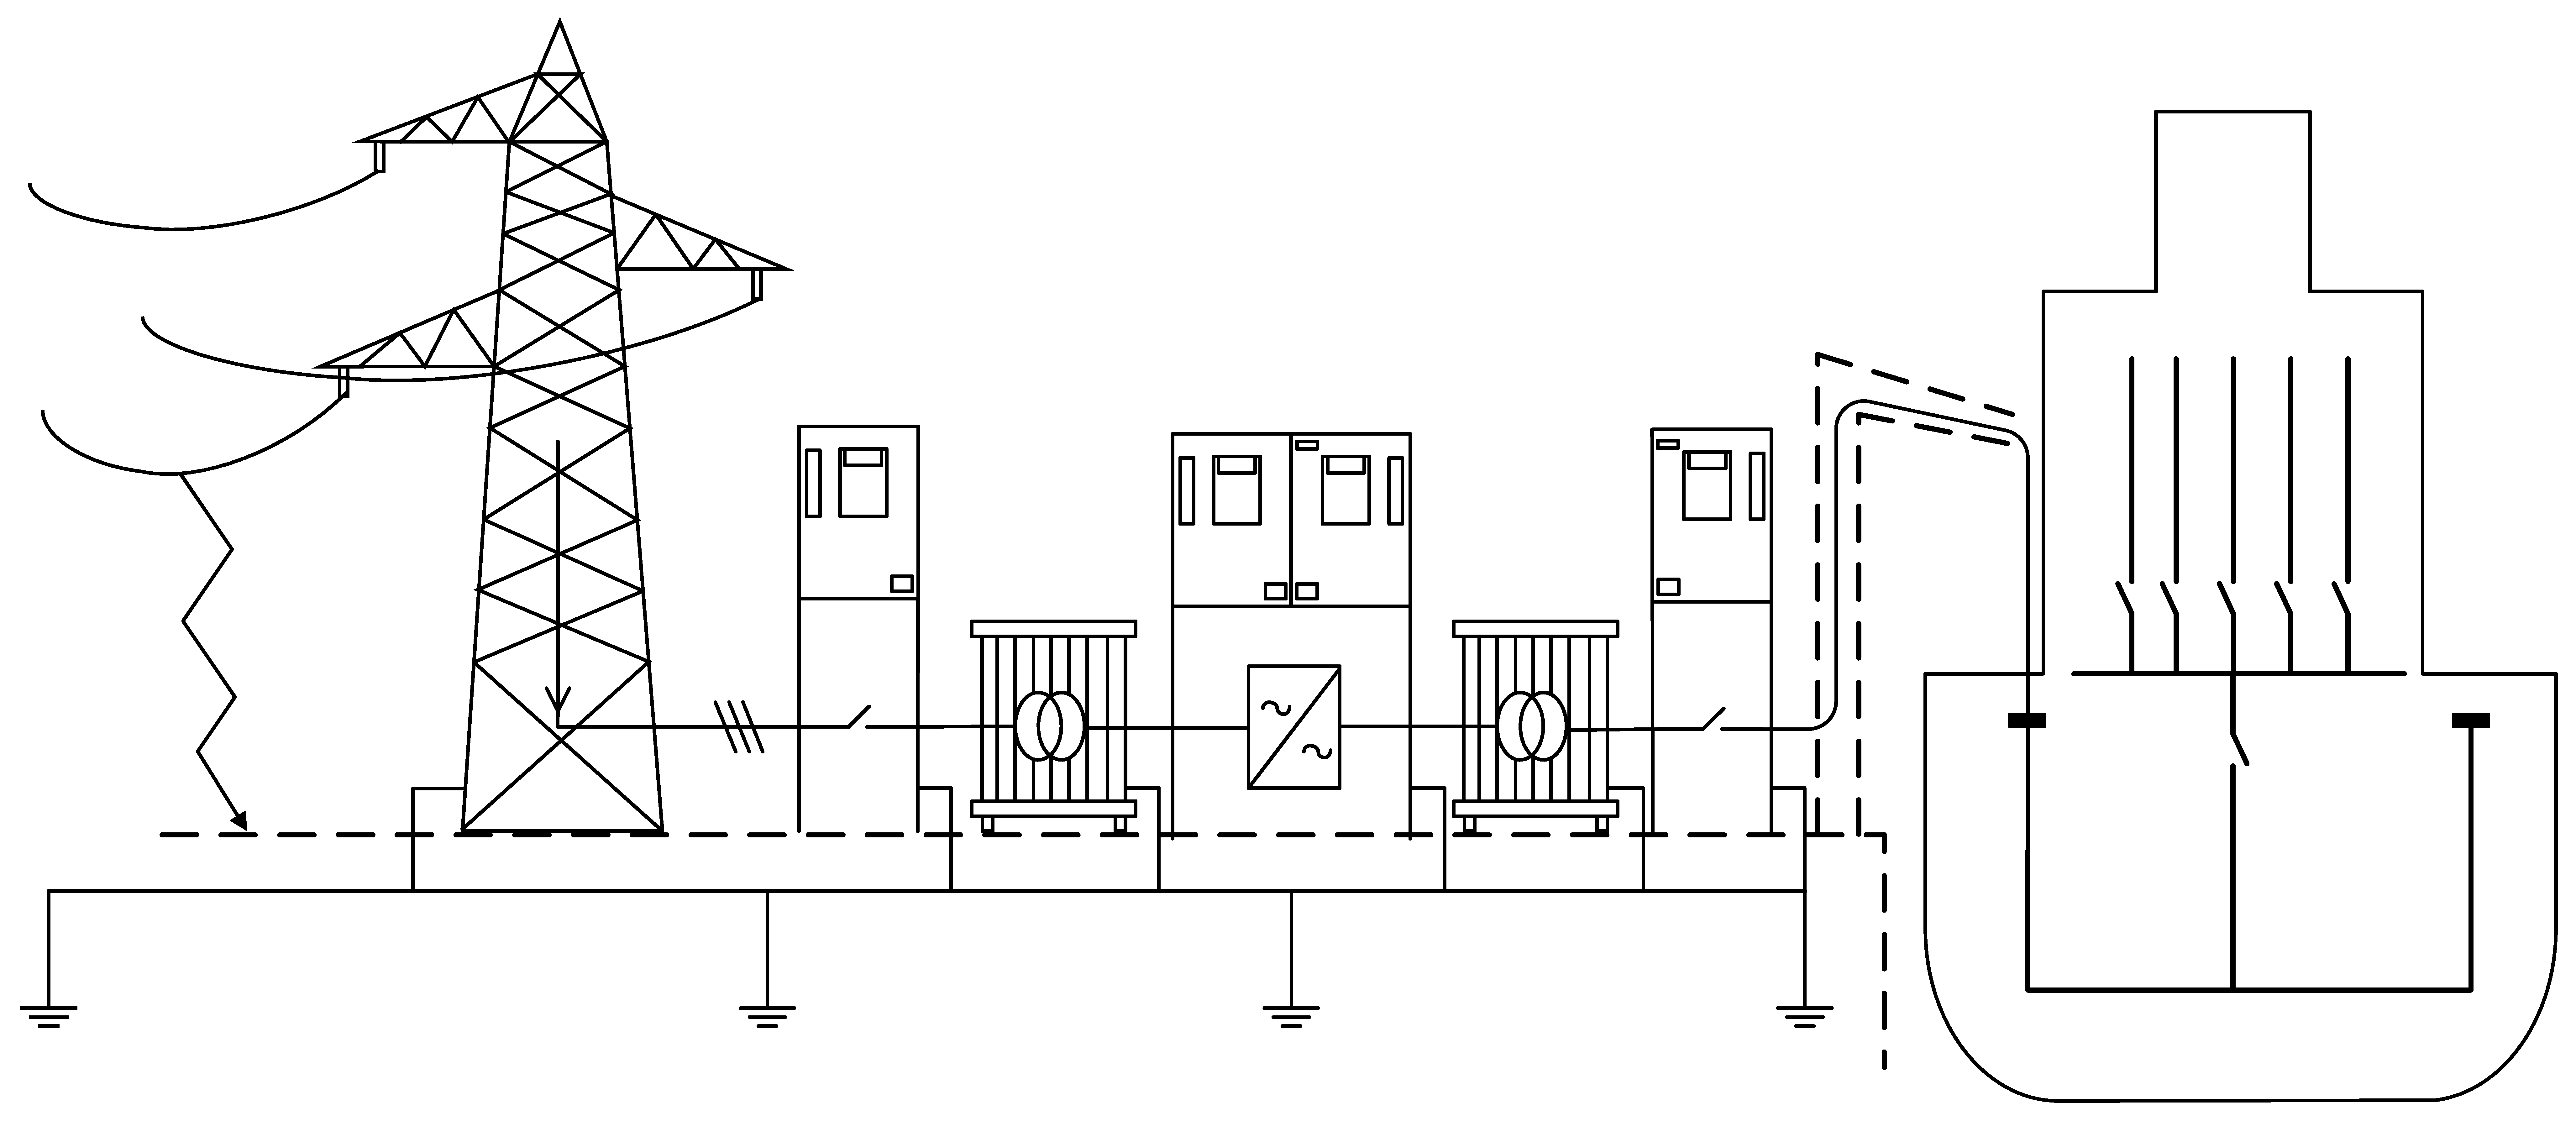
\includegraphics[width=0.95\textwidth]{高压船岸连接示意图.pdf}
	\caption{船岸连接示意图}
	\label{fig:船岸连接示意图}
\end{figure}


\section{船岸连接系统的配置方式}

\subsection{船岸连接高压岸电供电系统}

\zhlipsum[1]

\begin{figure}[!htp]
	\centering
	\includegraphics[width=0.9\textwidth]{高压岸电系统.pdf}
	\caption{高压岸电供电系统}
	\label{fig:高压岸电供电系统}
\end{figure}



\subsection{船岸连接低压岸电供电系统}


\zhlipsum[2]

\begin{figure}[!htp]
	\centering
	\includegraphics[width=0.9\textwidth]{低压岸电系统.pdf}
	\caption{低压岸电供电系统}
	\label{fig:低压岸电供电系统}
\end{figure}



\subsection{船岸连接小容量岸电供电系统}

\zhlipsum[3]

\begin{figure}[!htp]
	\centering
	\includegraphics[width=0.9\textwidth]{小容量岸电系统.pdf}
	\caption{小容量岸电供电系统}
	\label{fig:小容量岸电供电系统}
\end{figure}



\subsection{船岸连接不同方案对比}


% \begin{table}[!htp]
% 	\centering
% 	\caption[船用岸电供电方式比较]{船用岸电供电方式比较}
% 	\label{tab:船用岸电供电方式比较latex}
% 	\resizebox{\textwidth}{!}{%
% 	\begin{tabular}{cccc}  
% 	  \toprule
% 	    & 低压岸电/低压船舶     & 高压岸电/低压船舶        & 高压岸电/高压船舶  \\ 
% 	  \midrule
% 	  岸上系统电压/kV & 0.44          & 6~20             & 6.6/11     \\
% 	  船舶配电电压/kV & 0.44          & 0.4              & 6.6/11     \\
% 	  港口电网频率/Hz & 60            & 50               & 60         \\
% 	  船舶用电频率/Hz & 60            & 50               & 60         \\
% 	  岸电接入方式    & 港口提供电缆        & 港口提供电缆           & 船方提供电缆     \\
% 	  船舶改造复杂性   & 较小            & 较复杂,需要船舶上安装降压变压器 & 较小         \\
% 	  供电操作难易度   & 较复杂,需接驳船和多根电缆 & 较容易,仅需一根电缆       & 较容易,仅需少量电缆 \\
% 	  \bottomrule %添加表格底部粗线
% 	\end{tabular}
% 	}
% \end{table}


\zhlipsum[4]


\begin{table}[!htp]
	\centering
	\caption[船用岸电供电方式比较]{船用岸电供电方式比较}
	\label{tab:船用岸电供电方式比较}
	\resizebox{\textwidth}{!}{%
	\begin{tabular}{c}
		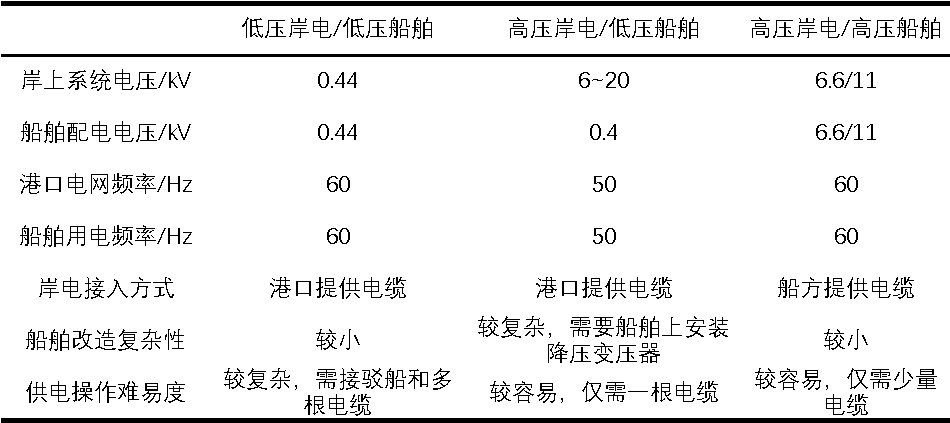
\includegraphics{船用岸电供电方式比较.pdf} 
	\end{tabular}
	}
\end{table}




\section{船岸连接系统面临的问题}
\subsection{船舶岸电供电并网切换解决处理方案}
\subsubsection{主动并网切换}
\subsubsection{被动并网切换}

\subsection{并网负载转移方式}
\subsection{逆功率处理方案}
\subsection{逆功率产生机理}
\subsection{逆功率的处理}
\subsection{不同控制方案简单对比}




\subsection{岸船连接段系统压降解决方案}

\subsubsection{隔离变压器的压降问题}
\subsubsection{输出电缆的压降问题}


\subsection{三相输出电压平衡控制技术}
\subsection{船岸等电位处理方案}


\zhlipsum[5]

\section{本章小结}


\zhlipsum[6]